\documentclass[11pt]{article}

\usepackage{graphicx}
\usepackage{amsfonts}
\usepackage{amsmath}
\usepackage{amsthm}
\usepackage{latexsym}
\usepackage{amssymb}
\usepackage{hyperref}

\newtheorem{theorem}{Theorem}[section]
\newtheorem{lemma}[theorem]{Lemma}
\newtheorem{corollary}[theorem]{Corollary}
\newtheorem{assumption}[theorem]{Assumption}
\newtheorem{proposition}[theorem]{Proposition}
\newtheorem{observation}[theorem]{Observation}
\newtheorem{defin}[theorem]{Definition}
\newtheorem{definition}[theorem]{Definition}
\newtheorem{example}[theorem]{Example}
\newtheorem{conjecture}[theorem]{Conjecture}
\newtheorem{claim}{Claim}

\pagestyle{plain}
\bibliographystyle{plain}

\title{K-Means Clustering}

\begin{document}

\maketitle
}
\section{Introduction}
\subsection{Clustering}
Clustering can be considered the most important unsupervised learning problem; so, as every other problem of this kind, it deals with finding a structure in a collection of unlabeled data.
A loose definition of clustering could be “the process of organizing objects into groups whose members are similar in some way”.


A cluster is therefore a collection of objects which are “similar” between them and are “dissimilar” to the objects belonging to other clusters.\cite{source}
We can show this with a simple graphical example:

\begin{figure}\begin{center}
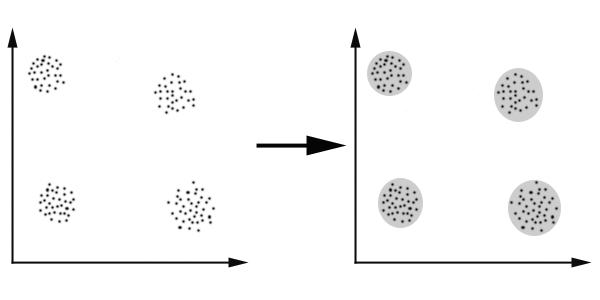
\includegraphics[scale=0.5]{clustering.jpg}
\end{center}

\end{figure}

\subsection{what is good clustering}
In order to get quality clusters, better clustering methods should be implimented which should have high Intra-class similarities ( All the data points in that cluster should be similar to each others) \\
and should have Low-inter class similarity ( all the clusters should be dissimilar to each other)\\
Inorder to check if the clustering method is appropriate, we need to check for the following characteristics:\\
\\
1.Similarity measure used by the mothod\\
2.Implimentations\\
3.Ability to discover some or all hidden patterns

\subsection{Good Clustering Algorithm}
A good Clustering algorithm should satisfy the following requirements.\\
1. Scalability, it should be able to cluster the entire data given but not just a part of it.\\
2. It should have the ability to deal with all kinds of attributes like Numerical, Binary, etc.\\
3. It should be able to deal with noisy and outlier data ( data point which is away from the clusters )\\

\section{Clustering Methods}

\subsection{Partitioning Method}
Clustering is based on data partitions which means it helps to discover the groupings in the data by optimizing a specific objective function and iteratively improving the quality of partitions\\
\subsection{Hierarchial Method}
finding new clusters using previously found ones. There are two approaches in this.\\
\subsubsection{Agglomerative method
}\\
Bottom- up-approach
If a set of points are considered in a Euclidean space. each data point is initially  in a cluster of its own.at each step by finding the two closest clusters, the two clusters are merged into a single cluster.\\
The key operation of Hierarchy agglomerative clustering is to repeatedly combine the two nearest clusters in to a larger cluster.\\
The process stops when all groups are merged to one or k number of clusters are formed.\\



\begin{figure}\begin{center}
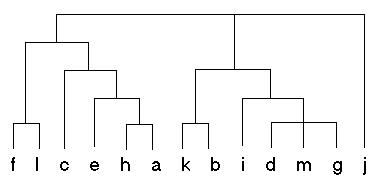
\includegraphics[scale=0.5]{Hierarch.jpg}
\end{center}

\end{figure}



\subsubsection{Divisive method}
 bottom up approach.\\
It is the opposite to Agglomerative method. In this all the data points are in a single cluster to begin with and the cluster is recursively split into small clusters,\\
Stops when the K number of clusters are formed.\\
\subsection{Density based method
}\\
clustering is based on density which means the regions with sufficiently high density points.\\
It discovers clusters of arbitrary shapes\\
\subsection{Model based method}\\
For this type of clustering,model hypothesis is done for each cluster and tries to find the best fit of \\
that model to each other.\\
\subsection{Constraint based method:}
  Clustering is done based on user specified constrains or some specific constraints


\section{Applications}\\

\subsection{Marketing:}\\ Marketing uses clustering technique to cluster the customer with high salary and target on  them. i.e., when a manager in bank wants to offer loans to their customers. they will collect the information of their customers with high salary and concentrate on them.

\subsection{Biology:}\\  Plants and animal are clustered into two different groups based on  their features

\subsection{ Libraries:}\\ Grouping similar books or books of same subjects at a place in order to identify them easily

\subsection{Insurance:}\\ To identify a group of car insurance policy holders with a high average claim cost

\subsection{Earthquake studies:}\\  clustering helps earthquake epicenters to identify places where earthquakes frequently happen

\subsection{WWW:}\\  In world wide web Clustering helps to identify all the documents related to the topic which was searched.

\subsection{Land use:}\\  clustering  helps to identify two or more land which are used for the same purpose by referring earth observation database



\section{K-Means Clustering}\\

K means is one of the best known clustering algorithm to solve the unsupervised learning issue. Assume a data set with ‘n’ data points x i , i=1...n that have to be partitioned 
into k clusters and the goal is to assign each data point to the nearest cluster. The aim of the algorithm is to find the positions "$ \mu $i" , i=1...k of the clusters that minimize the 
distance from the data points to the cluster centers $ \mu $i . Here, $ \mu $i i=1...k  are the centroids of the K clusters which are fixed a priority.\\
\\
Initialise a centroid (center) point for one for each cluster that is denoted by $ \mu $ . These centers should be chosen randomly in such a way that the each center is possibly far away from each other . Because the number of clusters 
and the cluster position might alter the final solution.\\
\\
After determining the centroids for each cluster , all the data points should be assigned to the centroid in such a way the 
distance between the centroid and data point is minimum.\\
\\
That means each point is assigned to the closest centroid and that collection of the points that are assigned to the centroid forms
a cluster.The centroids are updated based on the data points that belong to the cluster. Then all the data points are again assigned to the newly updated centroids and thus it changes the
initial cluster positions. After forming the new clusters the centroids are again updated . The assigning and updating the centroids are repeated until no data point changes in the cluster
or the centroid position remains the same.\\
\\
This  algorithm  aims at  minimizing  an objective function known as squared error function given by:\\  

\\
Formula pic.1
\\

'\mid\mid x_i-$ \mu $_j\mid\mid' is the Euclidean distance between xi and $ \mu $_j.\\

‘ki’ is the number of data points in ith cluster\\

‘k’ is the number of cluster centers.\\



\begin{figure}\begin{center}
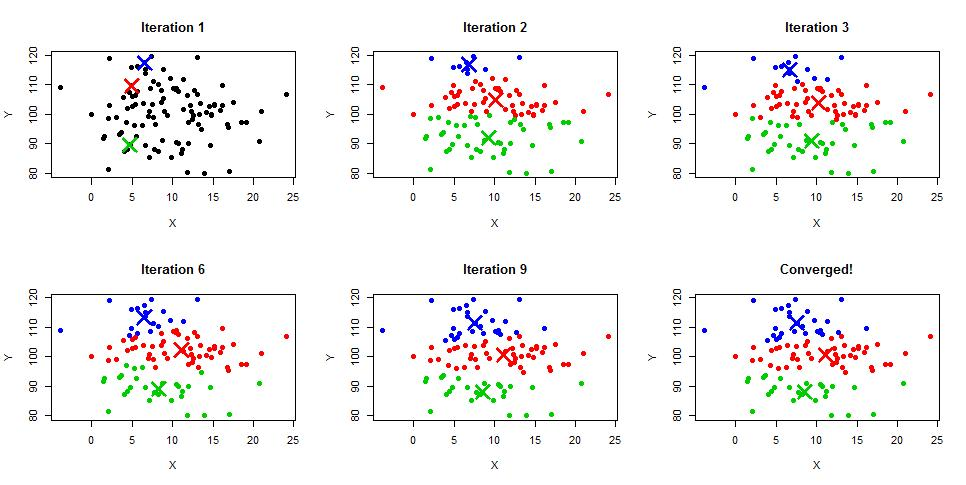
\includegraphics[scale=0.5]{sk1.jpg}
\end{center}

\end{figure}


1.In the below example , there are n data points . Three random centroids are chosen from the n data points i.e., k= 3 . Then the nearest data points are assigned to each centroid thus forming a new cluster shown in iteration.\\

 The Step by step iteration of the k-means algorithm is shown in the above diagram:\\

2. The centroids are then updated based on the data points in the cluster. The assignment of data points to the newly updated centroids is shown in iteration.\\
3. This process is repeated until convergence. That means this process is repeated until the data points in the clusters are constant or the updated centroid position is constant. The last iteration shows the final cluster output. 

\subsection{ALGORITHM:}

Step 1: Initialise 'k' number of clusters and the cluster centroids $ \mu $_1,$ \mu $_2, $ \mu $_3....$ \mu $_k  \textup{randomly.}\\
Step 2: Repeat\\
Step 3: \textup{Assign  each  data  point  to} $ \mu $_i ,i =1...k \textup{ such  that  the  distance  between  the  centroid  and }\\
\textup{ the  data  points  is  minimum  among the k clusters.}\\
Step 4:\textup{Recalculate  the  mean  for  each  cluster} \textup{based  on  the  data  points  assigned  to  the  cluster.}\\

\subsection{mean}\\

Formula\\

where, ki represents number of data points in ith cluster.\\

Step 5: Repeat the algorithm until no change.\\

\subsection{ASSIGNING POINTS TO THE CLOSEST CENTROID:}\\
To assign points to the closest centroid in the k-means algorithm often the Euclidean Distance measure is used for the data points in Euclidean space.\\
There are many other proximity measures other than Euclidean distance. Manhattan Distance can also be applied to measure the distance for the Euclidean Data. 
\subsection{EUCLIDEAN DISTANCE FORMULA :}\\

 For n dimensional data ,
MEAN COMPUTATION AND OBJECTIVE FUNCTION:
Mean Computation is nothing but calculating the centroid for each cluster. The data points that belongs to the cluster might alter at every step.So, the mean value changes at every single iteration.\\
Example : Consider three data points (x1,y1),(x2,y2),(x3,y3) which are two dimensional that belongs to one cluster.\\
Then the mean μ for the cluster is ,$\mu$ = ((x1+x2+x3)/3 , (y1+y2+y3)/3)
Using the above formula the mean is calculated in every step of the k-means clustering algorithm.


\subsection{OBJECTIVE FUNCTION OR THE SQUARED ERROR FUNCTION:}\\

The objective function measures the quality of the clustering . The aim of the algorithm is to minimise the Squared error function or the Objective function. For the squared error function\\
the error of each data point i.e., its euclidean distance from its nearest centroid is calculated and then total sum of the squared errors is computed. When there are two different\\
sets of clusters that are produced by two different runs of K-means , the one with smallest squared error distance is prefered because the centroids for those clusters with\\
minimum squared error distance have better representation of the points in their particular clusters.

\end{document}
